\begin{figure}[b!]
  \vspace{-1.5em}
  \centering
  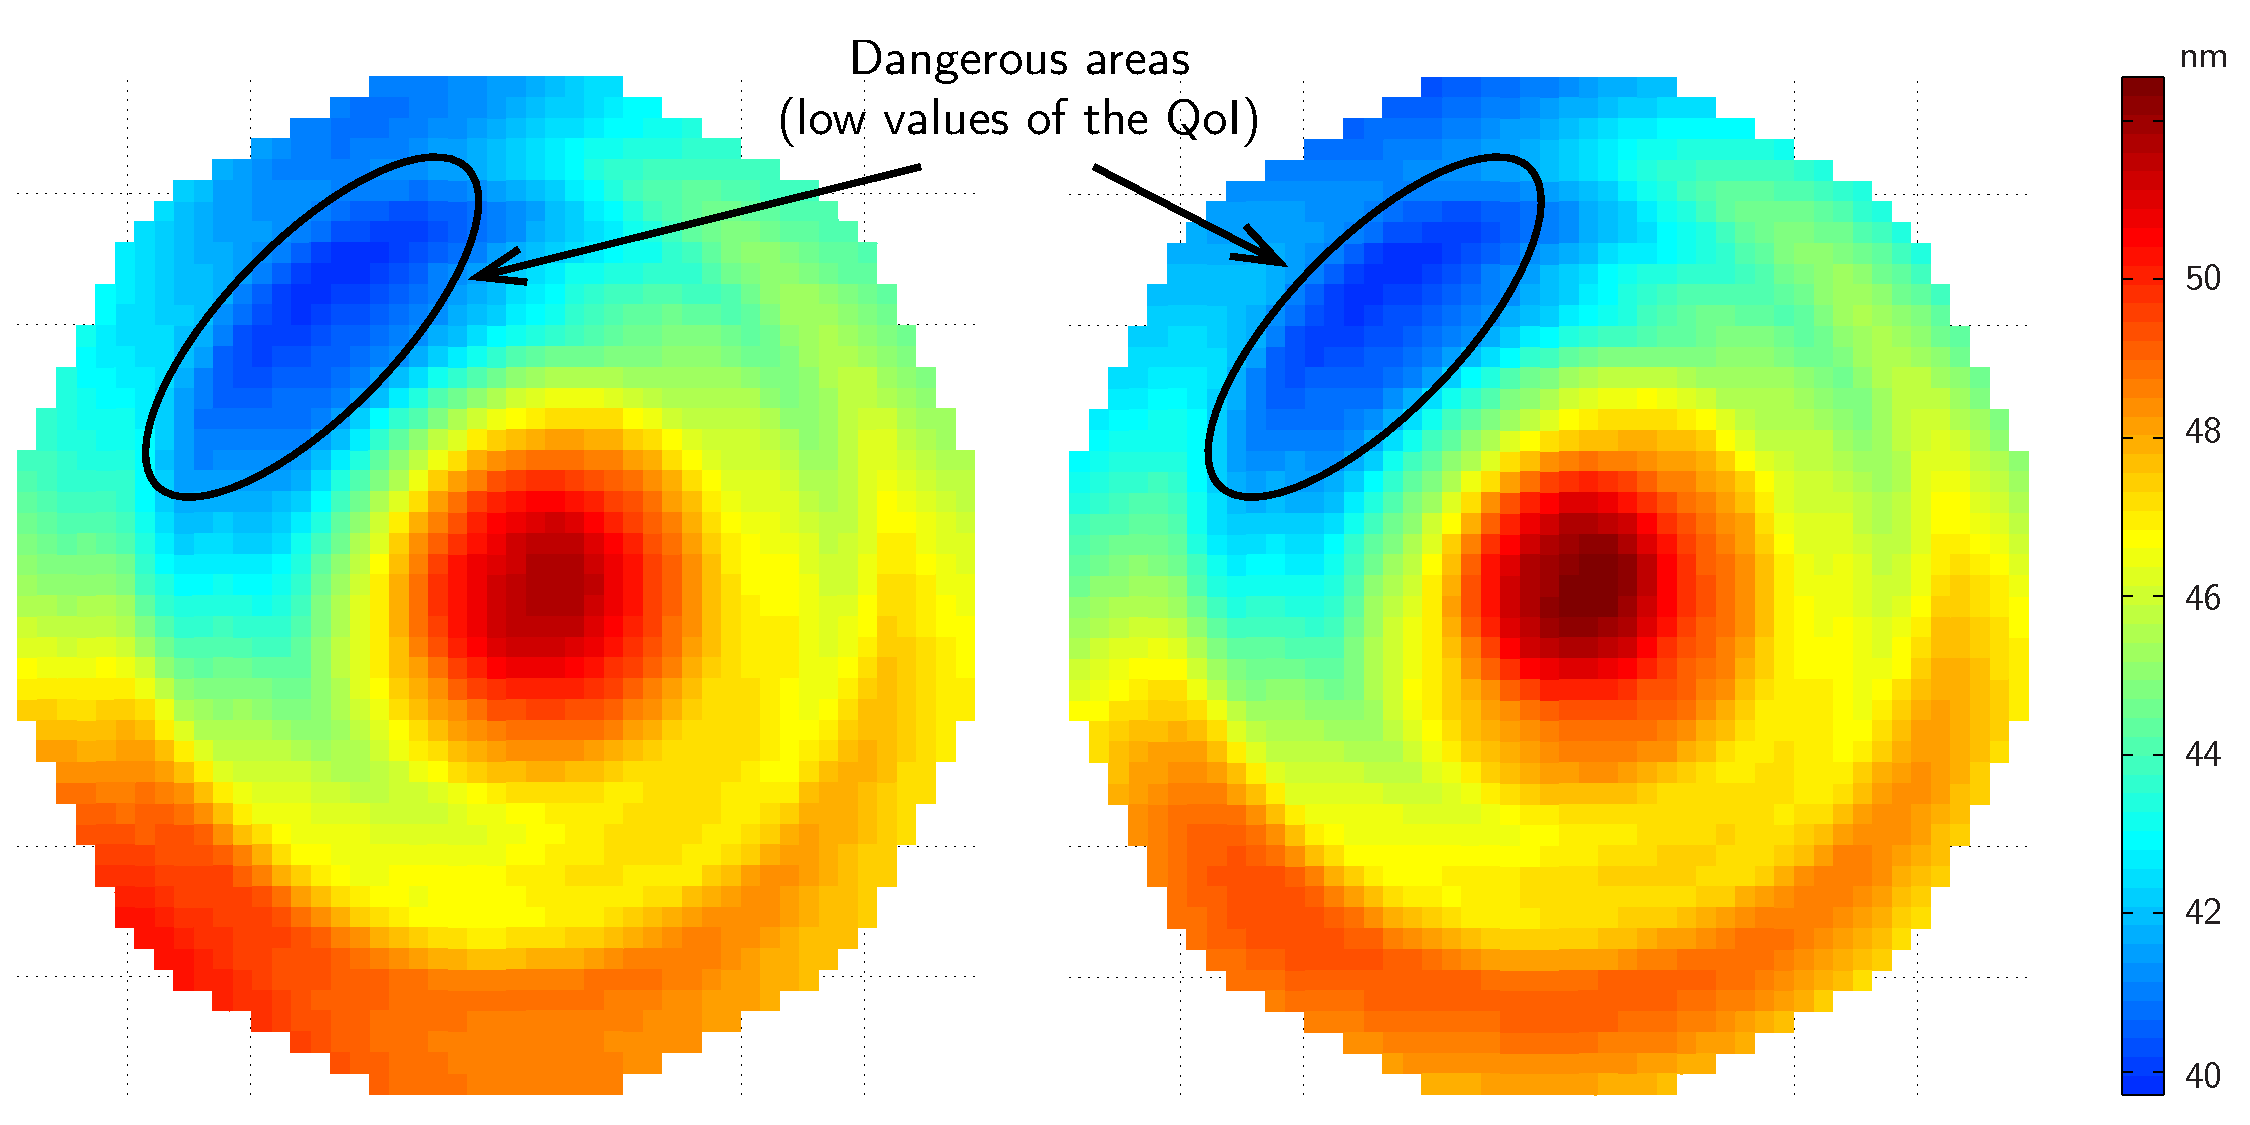
\includegraphics[width=1\linewidth]{include/assets/wafer-qoi.pdf}
  \caption{The true (on the left) and inferred (on the right) distribution of the QoI across the wafer.}
  \flabel{wafer-qoi}
\end{figure}

Let us consider an example that illustrates a particular application of the proposed technique. As previously mentioned, due to process variation, the key parameters that have direct impacts on power and temperature are intrinsically uncertain. Let $\u$ be one of such uncertain quantities; say, the effective channel length. Assume the manufacturing process imposes a lower bound $\u_*$ on the parametrization $\u$. This lower bound separates defective dies ($\u < \u_*$) from those that function properly ($\u_* \leq \u$). Possible actions that one might wish to take with respect to a single die on the wafer are: (a) keep the die if it closely conforms to the specification; (b) throw away the die if it exhibits an unacceptable divergence, due to process variation, from the specification. Let the distribution of $\u$ across the wafer be the one depicted on the left side of \fref{wafer-qoi} where 316 dies, four cores each, are placed in a $20 \times 20$ grid, and the gradient from navy to dark red represents the transition of $\u$ from low to high values.\footnote{The experimental setup is described in \sref{experimental-results} in detail.} A common approach to find this distribution is to deploy adequate test structures on the dies and measure $\u$ directly; then, the corresponding decision can be taken based on the collected information. The problem in this scenario, however, is that the described procedure is typically highly expensive to undertake.

The technique that we propose and develop in this paper operates on cheap, indirect measurements and, therefore, can considerably decrease the above-mentioned costs since no additional on-die test structures are required. The result of our framework applied to a data set, corrupted by noise, corresponding to only 20 spatial locations on the wafer (out of 316) is shown on the right side of \fref{wafer-qoi}. It can be seen that the fields closely match each other. Further, the technique can readily be utilized to estimate probabilities of various events, \eg, $\probabilityMeasure(\u < \u_*)$. This fact is especially advantageous since, in reality, we do not know the true values and, therefore, can reason about our decisions only in terms of probabilities. We can then reformulate our decision rule as follows: (a) keep the die if $\probabilityMeasure(\u_* \leq \u)$ is larger then a certain threshold; (b) throw the die away, otherwise. An illustration of this decision process is given in \fref{wafer-defect} where the threshold is set to two standard deviation below the mean value of $\u$, the circles mark defective dies (the navy areas in \fref{wafer-qoi}), and the gradient from light gray to red corresponds to the inferred probability of a die to be defective. It can be seen that the inference accurately detects faulty regions.
\begin{figure}[t!]
  \centering
  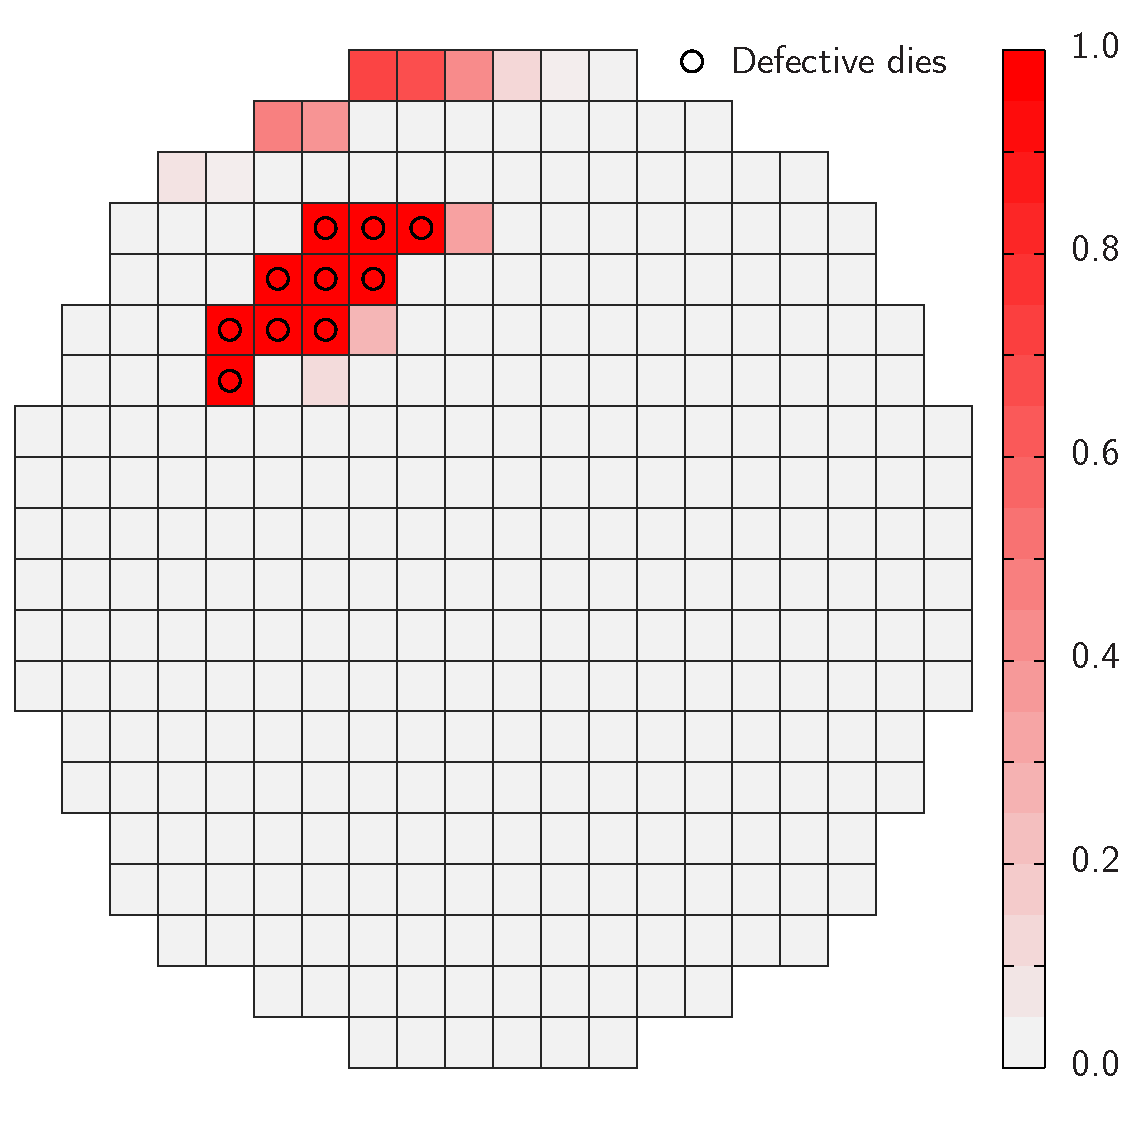
\includegraphics[width=0.7\linewidth]{include/assets/wafer-defect.pdf}
  \caption{Inferred probability of defective dies.}
  \flabel{wafer-defect}
  \vspace{-1.5em}
\end{figure}


In addition, we can introduce a trade-off action: (c) expose the die to a thorough inspection (\eg, via a test structure) if the threshold of (a) is no reached, and (b) has a separate threshold, which is also not satisfied. In this case, we can save money by examining only those dies for which there is no strong evidence of their satisfactory or unsatisfactory condition. Furthermore, one can introduce into play a so-called utility function, which, for each combination of an outcome of $\u$ and a taken action---(a), (b), and (c) in our example---assigns the corresponding amount of gain that the decision maker receives. Then, the inference path taken in this paper (Bayesian inference) can deliver such an action that maximized the expected utility with respect to the posterior distribution of $\u$; in other words, all possible outcomes of $\u$ weighted by their probabilities will be taken into account in the final decision.
